\iffalse
\let\negmedspace\undefined
\let\negthickspace\undefined
\documentclass[journal,12pt,twocolumn]{IEEEtran}
\usepackage{cite}
\usepackage{amsmath,amssymb,amsfonts,amsthm}
\usepackage{algorithmic}
\usepackage{graphicx}
\usepackage{textcomp}
\usepackage{xcolor}
\usepackage{txfonts}
\usepackage{listings}
\usepackage{enumitem}
\usepackage{mathtools}
\usepackage{gensymb}
\usepackage{comment}
\usepackage[breaklinks=true]{hyperref}
\usepackage{tkz-euclide} 
\usepackage{listings}
\usepackage{gvv} 
\usepackage{verbatim}                                       
\def\inputGnumericTable{}                                 
\usepackage[latin1]{inputenc}                                
\usepackage{color}                                            
\usepackage{array}                                            
\usepackage{longtable}                                       
\usepackage{calc}                                             
\usepackage{multirow}                                         
\usepackage{hhline}                                           
\usepackage{ifthen}                                           
\usepackage{lscape}
\newtheorem{theorem}{Theorem}[section]
\newtheorem{problem}{Problem}
\newtheorem{proposition}{Proposition}[section]
\newtheorem{lemma}{Lemma}[section]
\newtheorem{corollary}[theorem]{Corollary}
\newtheorem{example}{Example}[section]
\newtheorem{definition}[problem]{Definition}
\newcommand{\BEQA}{\begin{eqnarray}}
\newcommand{\EEQA}{\end{eqnarray}}
\newcommand{\define}{\stackrel{\triangle}{=}}
\theoremstyle{remark}
\newtheorem{rem}{Remark}
\begin{document}
\bibliographystyle{IEEEtran}
\vspace{3cm}
\title{11.9.4.4}
\author{EE23BTECH11027 - K RAHUL$^{*}$% <-this % stops a space
}
\maketitle
\newpage
\bigskip
\renewcommand{\thefigure}{\theenumi}
\renewcommand{\thetable}{\theenumi}
\textbf{Question:} \\
Find sum to n terms of the following series:\\
$\frac{1}{1 \times 2} + \frac{1}{2 \times 3} + \frac{1}{3 \times 4} + \ldots$
\bigskip \bigskip

\fi
\solution
\begin{table}[ht]
\setlength{\arrayrulewidth}{0.3mm}
\setlength{\tabcolsep}{15pt}
\renewcommand{\arraystretch}{1.5}



\begin{tabular}{ |p{1cm}|p{2cm}|p{2cm}| }
\hline
Symbol & Description & Value\\
\hline
$x\brak{n}$ & $n^{th}$ term of series & $\frac{1}{\brak{n+1}\brak{n+2}} u\brak{n}$\\
\hline
$y\brak{n}$ & Sum of $n$ terms of series & ?\\
\hline
%$x(l)$ & Last($l^{th}$) term of series & 350\\
%$x(0)$ & Starting ($0^{th}$) term of series & 17 %\\
%\hline
%d & Common difference of AP & 9\\
%\hline
\end{tabular}
\caption{Parameters}
 %Table 1: Parameters



\end{table}
\begin{align}
x\brak{n} &= \frac{1}{\brak{n+1}\brak{n+2}}u\brak{n}\\
& = \brak{\frac{1}{n+1} - \frac{1}{n+2}}u\brak{n}
\end{align}
Using \eqref{11027_when_c_not_1} and \eqref{11027_when_c_equals_1}, we get,
\begin{align}X\brak{z} &= -z log\brak{1-z^{-1}} + z^2 \log\brak{1-z^{-1}} + z\\
&= z\brak{z-1}\log\brak{1-z^{-1}} + z\\
    Y\brak{z} &= X\brak{z}U\brak{z}\\
     &=z^2\log\brak{1-z^{-1}} + \frac{z}{1-z^{-1}}
\end{align}
\begin{align}
	u\brak{n} &\system{Z} \frac{1}{1-z^{-1}} , \quad \abs{z} > 1\\
	u\brak{n+k} &\system{Z} \frac{z^k}{1-z^{-1}}, \forall k\in \mathbb{R}, \quad \abs{z} > 1 \label{Z_trans_pair}
\end{align}
Using \eqref{Z_trans_pair} and \eqref{11027_eq_log} ,
\begin{align}
    y\brak{n} &= u\brak{n+1} - \frac{1}{n+2}u\brak{n} , \; n \geq 0
\end{align}
Since $y(n)$ is only defined for $n \geq 0$, the above expression can be equivalently written as
\begin{align}
	y\brak{n} &= \brak{1-\frac{1}{n+2}} u\brak{n}
\end{align}
\newpage
\begin{figure}[h]
    %\caption{Stem Plot of $x\brak{n}$ v/s n}
    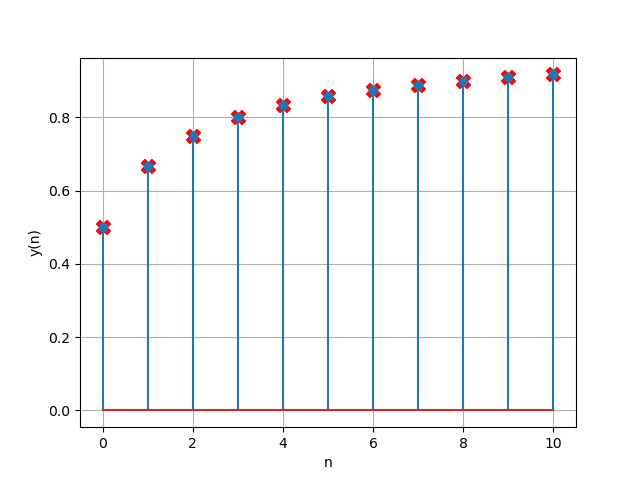
\includegraphics[width=0.3\textwidth]{ncert-maths/11/9/4/4/figs/y(n)_vs_n.png}\label{fig:stem-plot}
    \caption{Stem Plot of $y\brak{n}$ v/s n}
\end{figure}


